\documentclass{article}
\usepackage{blindtext}
\usepackage[utf8]{inputenc}
\usepackage{polski}
 \usepackage{geometry} 
 \usepackage{graphicx}
\newgeometry{tmargin=3cm, bmargin=3cm, lmargin=3cm, rmargin=3cm}
\renewcommand{\figurename}{Tabela}
\title{Sieć neuronowa MLP w problemie klasyfikacji ręcznie pisanych cyfr.}
\date{09 listopada 2017}
\author{Piotr Grzybowski}
 
\begin{document}
 
\maketitle
\newpage

\section{Opis problemu}
	Klasyfikacją możemy nazwać przypisanie każdego elementu z danego zbioru $X$ do dokładnie jednego z $k$ rozłącznych zbiorów $Y_k$. Przygotowane dane były reprezentowane przez ręcznie pisanych cyfr w postaci binarnych obrazów o rozmiarach $(10x7)$ pikseli, które były podzielone na dziesięć klas od zera do dziewiątki.
    
    
\section{Proponowane rozwiązanie}
	Powyżej zaprezentowany problem zostanie rozwiązany przy użyciu sieci neuronowej wielowarstwowej, użytej jako klasyfikator. 
	\subsection{Sieć neuronowa}
	Sieć neuronowa wielowarstwowa składa się z warstwy wejściowej, przynajmniej jednej warstwy ukrytej, warstwy wyjściowej. Każdy z neuronów takiej warstwy składa się z:
	\begin{itemize}
		\item Wektora wag o długości liczbie sygnałów wejściowych. Każdemu sygnałowi wejściowemu $x_i$, odpowiada dokładnie jedna kolejna waga $w_i$. Symbolicznie $W = [x_1, ..., x_N]$, gdzie N to liczba sygnałów wejściowych do neuronu.
		\item Stałej zwanej "biasem". Liczba rzeczywista.
		\item Funkcji aktywacji, według której obliczana jest wartość wyjścia neuronów w sieci neuronowej.
	\end{itemize}
    Wartość wyjścia neuronu jest liczona w sposób następujący (\textit{g} - funkcja aktywacji)
    \begin{equation}
    		Output = g(x^Tw + b)
    \end{equation}
    
	Poniżej krótki opis każdej z warstw uwzględnionych powyżej:
	\begin{itemize}
		\item \textbf{Warstwa wejściowa:} posłuży tylko jako miejsce do którego będziemy ładować dane, na których sieć będzie przeprowadzała operacje. Warstwa wejściowa charakteryzuje się tym, że ma takie samo wyjście jak wejście. W zakładanym modelu posłuży ona jako \textit{'data loader (ang.)}, czyli będzie przyjmować dane ze świata wewnętrznego, przechowywać je w trakcie przeprowadzania operacji oraz przesyłać wyście do kolejnej warstwy. Warstwa wejściowa składa się z $N$ neuronów, gdzie $N$ zależy od wymiarowości danych wejściowych. Przykładowo w naszym wypadku warstwa wejściowa będzie składała się z 70 neuronów wejściowych, gdyż binarny obraz o rozmiarze $(10x7)$ możemy zapisać za pomocą 70-cioelementowego wektora. 
		
	\item \textbf{Warstwa ukryta:} Składa się z $K$ neuronów, gdzie ich liczba jest zależna od użytkownika 
	
	\item \textbf{Warstwa wyjściowa: }Warstwa wyjściowa zawiera tyle neuronów, do ilu możliwych klas możemy przypisać nasze dane. Działa ona jako klasyfikator. Neuron z największą wartością aktywacji wskazuje na klasę, którą sieć zaklasyfikowała daną wejściową. 
	\end{itemize}
	
    
    \newpage
	\section{Zbiór danych}
	Zbiór danych został przygotowany przez studentów. Zawiera on 1744 przykłady ręcznie pisanych cyfr na czarno białym obrazie binarnym o rozmiarze (10x7). W procesie uczenie zostanie on podzielony na podzbiory rozłączne: treningowy, walidacyjny, testowy.
	
	\newpage
	\section{Badania}
	Podstawowym problemem w poprawności działania sieci neuronowej jest dobór odpowiednich hiperparametrów. W badaniach zbadane zostaną hiperparametry pod względem jakości predykcji jak i szybkości uczenia. Kolejnym problemem jest wybór sposobu optymalizacji funkcji kosztu. Kolejnym problemem jej przeciwdziałanie "overfittingowi", zbadana zostanie regularyzacja. 
	

	\subsection{Szybkość uczenia w przypadku liczby neuronów w warstwie ukrytej}
	W części tej została zbadana wymagana liczba epok do wyuczenia sieci neuronowej. Wyniki badań przedstawia poniższa tabela:
	
	\begin{figure}[h]
		\centering
		\caption{}
		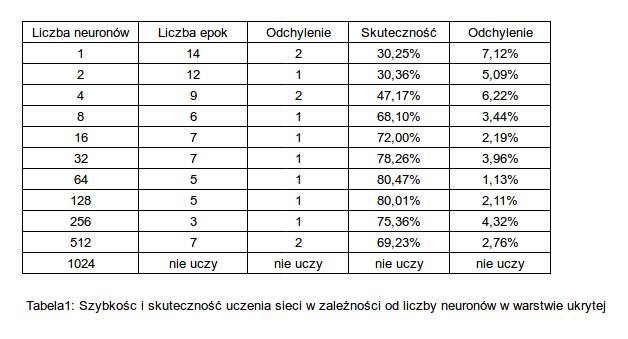
\includegraphics[width=0.5\textwidth]{tabela_liczba_neuronow.jpg}
	\end{figure}	 
	Na podstawie powyższej tabeli można stwierdzić, że zbyt mała liczba neuronów w warstwie ukrytej wymaga większej liczby epok do wyuczenia modelu. Charakteryzuje się także tym, że skuteczność predykcji nie jest wysoka, mała liczba neuronów zaczyna dokładnie odzwierciedlać zbiór treningowy (ang. overfitting), natomiast nie są one w stanie w dobry sposób reprezentować danych w zbiorze, który nie uczestniczył w procesie uczenia. Po drugie zbyt duża liczba neuronów w warstwie ukrytej powoduje, że liczba wymaganych epok się zwiększa, jeżeli natomiast będzie ich zbyt dużo do wielkości posiadanego zbioru uczącego możemy zauważyć zjawisko nie douczenia (ang. underfitting), model nie jest w stanie zapreprezentować dobrze nawet danych treningowych jeżeli jest ich niewystarczająco dużo.
	
	\subsection{Przebadanie różnych współczynników uczenia}
	W części tej została zbadana wielkość stałej uczenia w trakcie wyuczenia sieci neuronowej. Wyniki badań przedstawia poniższa tabela:
	
	\begin{figure}[h]
		\centering
		\caption{}
		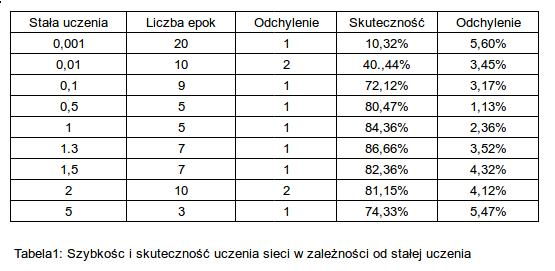
\includegraphics[width=0.5\textwidth]{tabela_stala_uczenia.jpg}
	\end{figure}	 
	Na podstawie powyższej tabeli można stwierdzić, że zbyt mała stała uczenia powoduje, że model może utknąć w minimum lokalnym jak i potrzebuje więcej epok aby wyuczyć się na danych treningowych. Z kolei zbyt duża stałą uczenia powoduje, że możemy oscylować wokół minimum funkcji kosztu i nigdy do niego nie trafimy, powoduje to, że nasz model osiąga gorsze wyniki niż oczekujemy. Kiedy stałą uczenia jest dużo za dużo model nie uczy się w cale, podobnie w przypadku zbyt małej dążącej do zera stałej uczenia.
	
	\subsection{Wpływ liczebności zbioru uczącego}
	W części tej została zbadana wielkość zbioru treningowego w trakcie wyuczenia sieci neuronowej. Wyniki badań przedstawia poniższa tabela:
	
	\begin{figure}[h]
		\centering
		\caption{}
		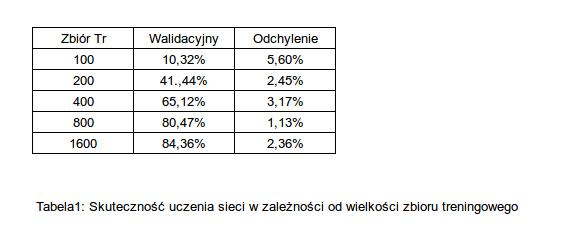
\includegraphics[width=0.5\textwidth]{tabela_zbior.jpg}
	\end{figure}	 
	Większy zbiór treningowy przeciwdziała overfittingowi. W naszym przypadku wymagana jest większa liczba danych do wyuczenia modelu do predykcji na wyższym poziomie. Powinno się zastosować proces Data Augumentation to generowania większej liczby danych, jednakże wykraczało to za ramy tego zadania. Z doświadczenia, zbyt duża liczba danych może spowodaować że model nie będzie się w stanie wyuczyć w akceptowalnym czasie bądź nigdy.
	
	\subsection{Metody optymalizacji}
	Przebadane zostały moteody optimalizacji gradientu prostego z dodatkiem momentum i bez. Momentum zapewnia nam szybsze zbieganie do minimum funkcji kosztu. W porównaniu do poprzednich eksperymentów, prrzy zastosowaniu momentum wystarczało do trzech epok przy 64 neuronach i współczynniku uczenia 1.3 aby szybko osiągac wyniki powyżej 80 procent na zbiorze walidacyjnym.
	   \newpage
	\subsection{Wpływ inicjalizacji wartości wag początkowych}
	W zadaniu zostały zbadane dwa sposoby initializowania wag. Pierwszym z nich było zastosowanie Rozkładu Normalnego o średniej równej 0.0 oraz odchyleniu standardowym 1.0. Wiąże się to jednak z tym, że wagi nie będą mocno zróżnicowane. Rozkład losowanych zmiennych będzie płaski:
	
	\begin{figure}[h]
		\centering
		\caption{}
		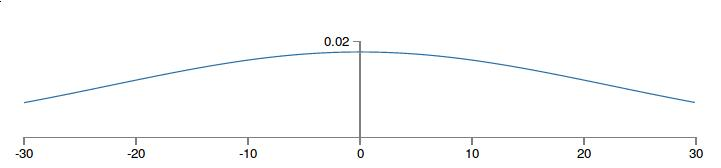
\includegraphics[width=0.5\textwidth]{gauss1.jpg}
	\end{figure}
	
	Lepszym sposobem będzie użycie Rozkładu Normalnego, z przeskalowanym odchyleniem standardowym o pierwiastek liczby neuronów w initializowanej warstwie. Spowoduje to, że rozkład losowanych zmiennych będzie bardziej zróżnicowany:
	
	 \begin{figure}[h]
		\centering
		\caption{}
		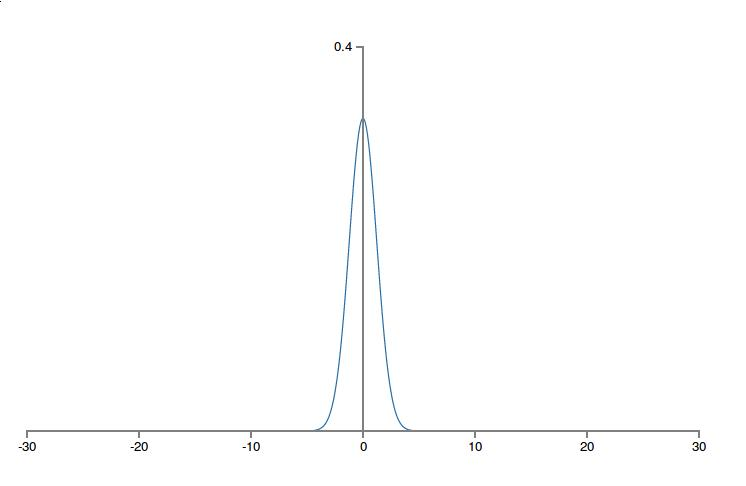
\includegraphics[width=0.5\textwidth]{gauss2.jpg}
	\end{figure}
	
	W przypadku drugiego rozkładu initializowanych wag uczenie przebiegało szybciej.
\newpage	
	\section{Podsumowanie}
	
	Uczenie sieci neuronowych jest pewną rodzaju sztuką. Można bardzo skrupulatnie dobierać hiperparametry, stosować różne funkcje kosztu, funkcji aktywacji, różnych metod optymalizacji co sprawia, że zadanie jest trudne. Jednakże warto korzystać także z pewnych wzorców i dobrych praktych, które będą działać poprawnie nawet dla naszych nowych problemów. 


\end{document}

